\chapter{系统总体设计}\label{chap:overal}

在进行系统设计时,首先需要了解 YOLO 算法的流程,再结合平台对具体的框架进行设计。对于CPU计算平台而言,设计方法相对简单,只需要处理好各运算之间的逻辑关系;而对于本次设计所采用的异构计算架构,还需要处理好各运算之间的顺序,以及运算的划分,从而获得最大的计算效率。考虑到 FPGA 和 CPU 不同的计算特性,需要对算法的运算进行合理的划分。对于计算密集型,运算之间数据关联性小的任务,适合使用 FPGA 进行并行加速,而一些串行,计算量较少的任务,则适合在 CPU 上完成。而在本文的任务中,还需要考虑 FPGA 硬件资源的问题,对任务进行合理划分。本章主要介绍系统的整体逻辑结构以及异构计算中任务划分的情况。

\section{系统设计内容及平台的选择}

本设计主要包含三个部分,RISC-V Core和卷积神经网络加速器,以及将两部分结合起来实现完整功能的SOC部分。卷积神经网络的硬件加速通常可以采用ASIC或者FPGA来实现,两者均是采用定制的硬件电路来加速算法。通常ASIC的性能更高,功耗更低,但是由于成本过高,因此在本设计中采用FPGA作为硬件平台。

由于一些 RISC-V 处理器缺少调试接口,不方便调试和下载程序,本文提出了一种在 ZYNQ 芯片上运行 Linux 系统与 RISC-V 处理器共享内存的方法来解决该问题。考虑各方面因素,最终选取了 PYNQ-Z2 作为硬件平台。 PYNQ-Z2 上使用Xilinx ZYNQ 7020芯片,芯片包含了 13,300 个可编程逻辑单元,每个逻辑单元有4个6输入查找表和8个触发器;芯片有 630 KB 的块存储器,220 个 DSP 运算单元,逻辑资源相对丰富;开发板引出数十个 IO 口和一个 HDMI 接口,拥有 512MB 的 DDR3,足够本系统使用。

\section{系统的任务划分}

% 在本文设计 CNN 加速器的过程中,首先需要对 CNN 模型进行分析,进行任务划分,针对各任务的不同特点,将任务划分为 FPGA 优化和 CPU 优化。任务划分的流程如图~\ref{fig:taskdiv}所示。

考虑到 FPGA 硬件资源的限制以及其运算特性,本文对 YOLO 算法进行了详细的分析,针对算法中不同的任务的运算特点,将其一些计算密集型的任务使用 FPGA 进行加速,而一些流程控制和计算量小的任务使用 RISC-V 处理器完成。具体的任务划分思路如图~\ref{fig:taskdiv}所示。

\begin{figure}[!htbp]
    \centering
    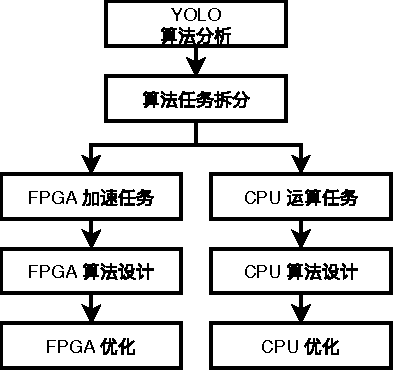
\includegraphics[width=0.40\textwidth]{taskdiv}
    \caption{任务划分流程}
    \label{fig:taskdiv}
\end{figure}

\begin{enumerate}
\item 首先对 CNN 模型进行分析,理解整个算法内部的逻辑以及数据流向。YOLO V2 算法主要有三个步骤:

    \begin{enumerate}
    \item 首先输入任意尺寸的 RGB 格式的图像,将各像素的值归一化到0-1之间,再将图像进行缩放到 $244 \times 244$ 大小,不改变图像的比例,不足处用 0.5 补充,这样就得到了 $244 \times 244 \times 3$ 的矩阵;
    \item 将(1)中得到的矩阵输入 Darknet 网络进行检测,网络检测后输出 $7 \times 7 \times 1024$ 的矩阵;
    \item 对网络输出的结果进行处理,获取输出的边框的信息,再根据各个边框的位置,可信度等,获得最有可能的边框位置。
    \end{enumerate}

\item 在这三个步骤中,步骤(1)的图像预处理和步骤(3)图像的后处理在整个计算中耗时不多,并且计算中设计到了指数运算,这部分如果使用 FPGA 加速需要消耗较多资源,性价比低,因此放在 CPU 上进行计算;
\item YOLO V2 算法中主要有3种类型的层:卷积层、池化层和重排序层。现有的研究表明,卷积层在神经网络的计算中占了大部分计算量,以 Alex-Net 为例,卷积层占了90\% \citep{chen2016eyeriss} 以上的计算量,使用 FPGA 对其并行加速是一种很有效的手段 \citep{farabet2009cnp,peemen2013memory,chen2014diannao}。池化层的运算过程与卷积层类似,不同的是卷积层中使用的是乘加运算而池化层中使用的是比较运算,因此本设计中选择将卷积层和池化层使用 FPGA 进行加速。重排序层的运算过程与内存搬运的过程类似,在 FPGA 中容易实现,因此重排序层也使用 FPGA 进行加速。
\end{enumerate}

\section{基于异构计算的系统体系结构}

考虑到图像的输入及数据存储设备,整个异构系统的结构如图~\ref{fig:system_structure}所示。整个算法运行的流程如下:图像及预训练的权重数据存储在外接的 SD 卡中,PS部分,CPU 通过 SD 卡控制器读取 SD 卡中的图像数据,对其进行预处理后,将其存储到 DDR 内存中;CPU 读取 SD 卡中的权重数据,将其存储在 DDR 内存中。神经网络算法加速器从 DDR 内存中读取预处理过的图像数据及权重数据,对图像进行运算,将运算的输出的结果矩阵存放到 DDR 中。最后 CPU 再从 DDR 中读取神经网络加速器的结果矩阵,进行图像的后处理,将标注完成的图像写回外置的的 SD 卡中。

\begin{figure}[!htbp]
    \centering
    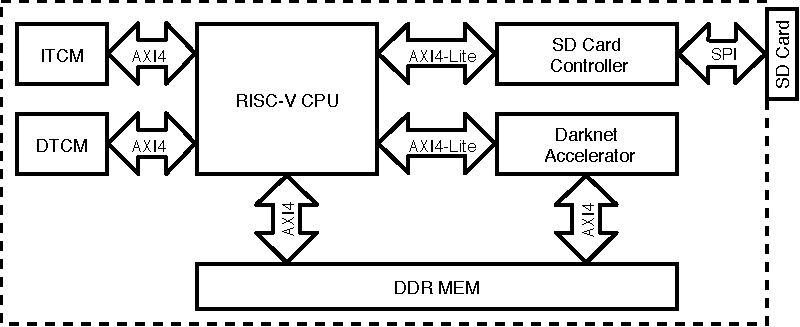
\includegraphics[width=0.70\textwidth]{system_structure}
    \caption{异构系统体系结构}
    \label{fig:system_structure}
\end{figure}

为了保证图像输出的连续性,本设计使用多级缓存,避免让 CPU 读取加速器正在写入的缓存区域。这样输出的实时性得到保证,提高了程序运行的效率。

\section{本章小结}

本章主要介绍了卷积神经网络加速器的总体架构设计,对 YOLO V2 算法进行了任务划分,规划了 SOC 的总体设计。在接下来的第四章和第五章会分别详细介绍 CNN 加速器的设计过程和 SOC 的设计过程。